Il existe de nombreuses manières d'accéder au Raspberry Pi. Nous détaillerons ici les principales.

\begin{figure}[h!]
\begin{center}
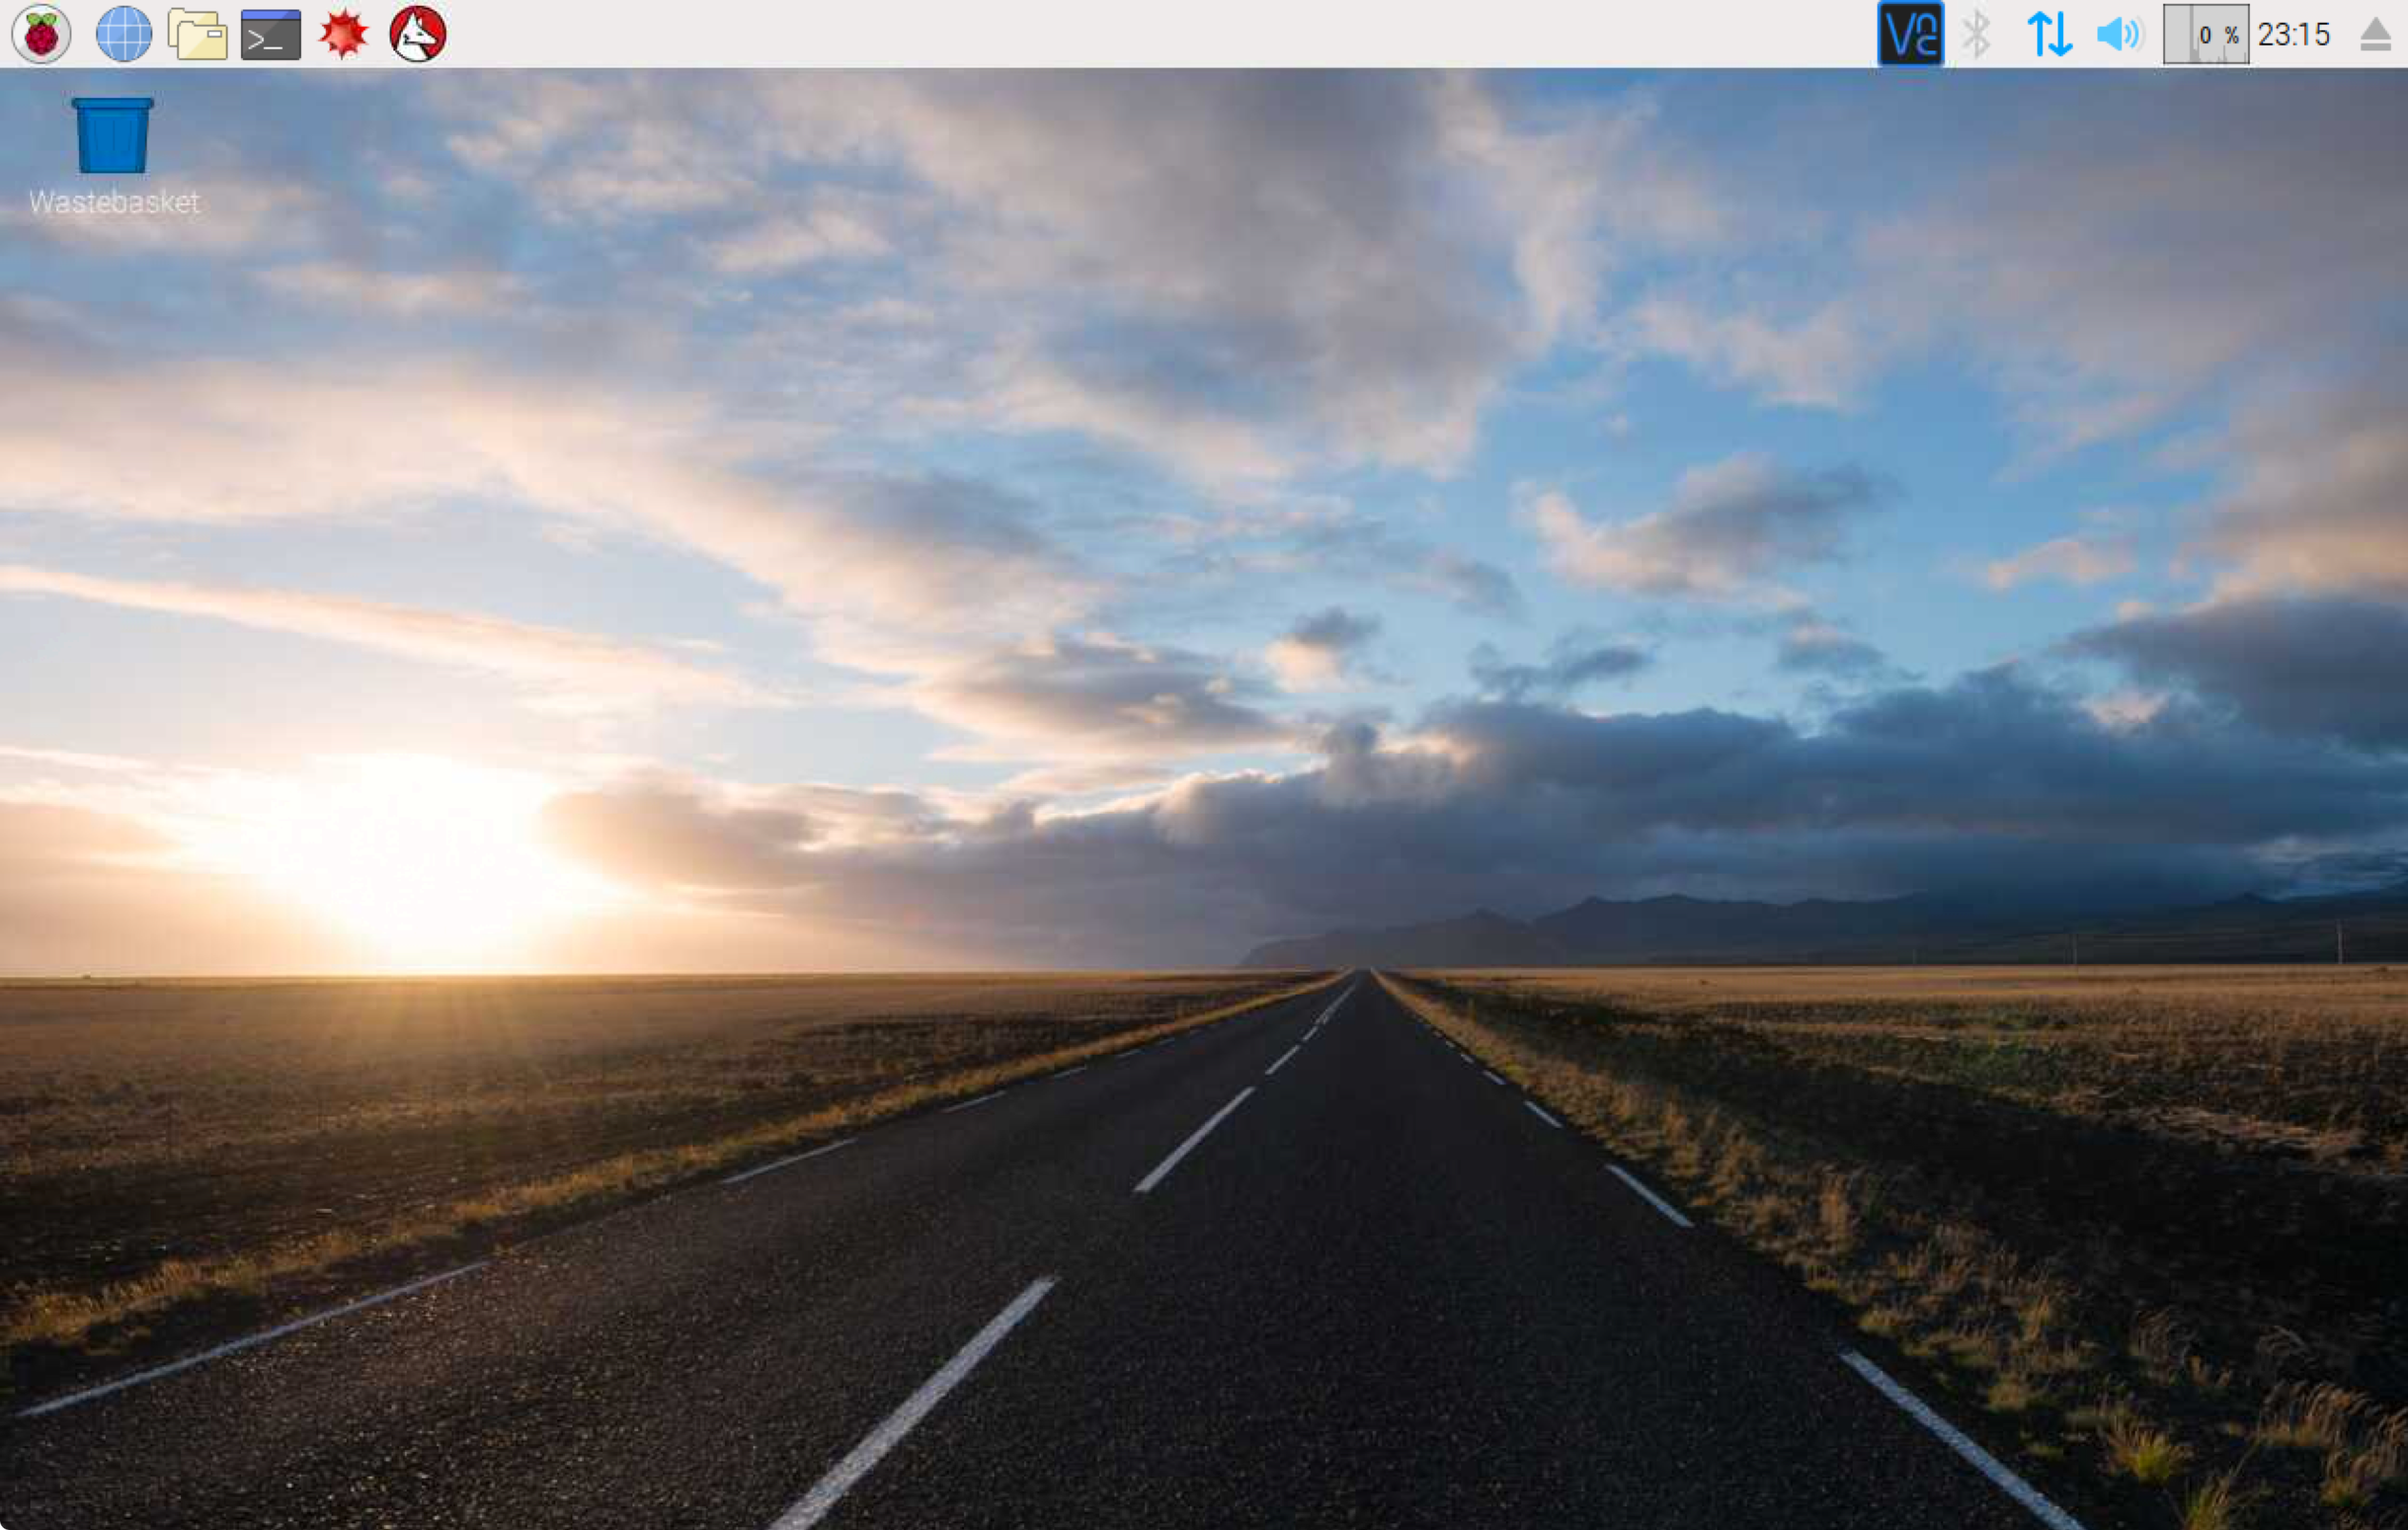
\includegraphics[width=15cm]{raspi.png}
\end{center}
\caption{Interface graphique du Raspberry Pi}
\label{interface}
\end{figure}

\subsection{Connexion directe}

La plus simple est bien sûr de se connecter à un écran via le port HDMI. La connexion est directe, et très fiable. Cependant, on n'a pas toujours un écran libre à disposition, et c'est là que les techniques de connexion suivantes pourront montrer leurs avantages.

\subsection{Connexion SSH (\textit{Secure Shell})}

Il s'agit ici de se connecter au terminal du Raspberry Pi. On n'aura pas accès à l'interface graphique, ce qui complique certaines opérations. Cependant, pour lancer un script ou mettre à jour quelques programmes, c'est un moyen rapide d'accéder au Raspberry Pi.

On se connecte au terminal du Raspberry Pi... par le terminal d'un autre ordinateur! Sur Windows, le programme s'appelle Console, sur macOS simplement Terminal. Une fois le programme ouvert, on trouve d'habitude une simple ligne de texte, et beaucoup d'espace dans lequel écrire des commandes.

Voici celle qui nous permet de nous connecter :

\texttt{ssh nom\_utilisateur@serveur}

Quand on configure le Raspberry Pi, un nom d'utilisateur par défaut est créé, il s'agit simplement de \texttt{pi}. Quant au serveur, ce peut-être une URL (une adresse, comme \texttt{raspberry.serveur.com} par exemple), ou bien une adresse IP (plus compliqué, il existe plusieurs types, mais on retiendra qu'il s'agit d'une suite de chiffres séparés par des points, comme ceci par exemple : \texttt{192.168.1.314}).

Nous vous aiderons à trouver l'adresse du serveur.

Une fois qu'on a l'adresse du serveur, on entre la commande, et un mot de passe est demandé. A nouveau, le Raspberry Pi en a un par défaut : \texttt{raspberry}.

On entre le mot de passe (il ne s'affiche pas, c'est tout-à-fait normal, il faut le taper à l'aveugle), et on a enfin accès au terminal du Raspberry Pi! Pour voir si tout fonctionne, essayez de taper la commande \texttt{uptime}. C'est le temps qu'est resté allumé votre Raspberry Pi depuis qu'on l'a branché à l'alimentation!

\subsection{Connexion VNC}

Ce type de connexion à distance est beaucoup plus agréable : on accède à l'interface graphique, mais via Internet, et non plus via un câble. Ce qui veut dire que si votre appareil est branché à Internet, vous pouvez potentiellement y accéder depuis n'importe où dans le monde!

Pour activer VNC sur le Raspberry Pi, il faut aller dans le terminal, et taper la commande \texttt{sudo raspi-config}. Puis sur l'interface qui s'affiche, on descend avec les flèches du clavier jusqu'à \texttt{Interfacing Options}. On valide avec la touche Entrée. L'option \texttt{VNC} apparaît, il suffit de l'activer.

On va aussi modifier la résolution tant qu'on y est. Il faut cette fois se rendre sur \texttt{Advanced Options} $\rightarrow$ \texttt{Resolution}. Une résolution de 1280x1024 devrait suffire!

\begin{figure}[h!]
\begin{center}
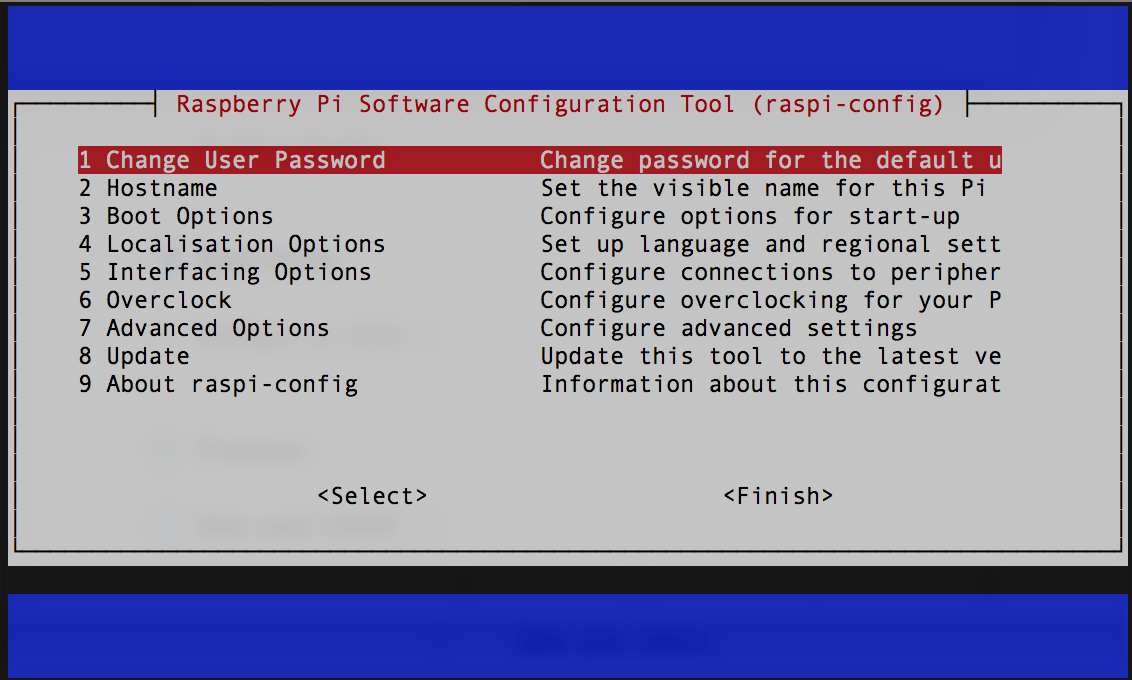
\includegraphics[width=8cm]{raspi-config.png}
\end{center}
\caption{raspi-config}
\label{raspi-config}
\end{figure}

C'est tout pour la configuration sur le Raspberry Pi! A partir de maintenant, plus besoin d'y toucher. Sur notre autre ordinateur maintenant, il faut télécharger un client VNC : \url{https://www.realvnc.com/en/download/vnc/}.

En lançant le programme VNC Connect, il nous est demandé l'adresse du serveur VNC. C'est la même que pour le serveur qu'on a du indiquer lors de la connexion SSH. Ensuite, une fenêtre s'ouvre pour demander l'utilisateur et le mot de passe. Rappelez-vous : par défaut, il s'agit respectivement de \texttt{pi} et \texttt{raspberry}.